\label{s:filtering_dtcwt}
%
\begin{figure}[t]
\centering
\begin{tabular}{@{}c c@{}} % @{} removes padding around the edge of the table
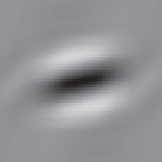
\includegraphics[width=0.2\columnwidth]{\figpath/filtering/dt_cwt_r4} &
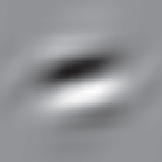
\includegraphics[width=0.2\columnwidth]{\figpath/filtering/dt_cwt_c4} \\
(a) & (b)
\end{tabular}
%
\caption{(a) Real and (b) complex filters for the $15^\circ$ subband of the \dtcwt{}.}
\label{f:filters_dtcwt}
\end{figure}%
%
The Dual-Tree Complex Wavelet Transform (\dtcwt{}~\cite{Kingsbury_ACHA01}) is a directionally selective representation that combines the strengths of approximately shift-invariant coefficient magnitudes and local phase information with the computational efficiency of decimation (\ie~downsampling the image rather than increasing the filter size). 

For a given pixel at a given scale, the \dtcwt{} combines the responses to a pairs of wavelets -- one real, one complex, and differing in phase by $90\deg$~(\fref{f:filters_dtcwt}) -- at six orientations: $\pm 15\deg$, $\pm 45\deg$ and $\pm 75\deg$. Because these filters are not exactly rotationally symmetric, the wave frequencies of the $\pm 45\deg$ sub-bands must be reduced so that they lie closer to those at $\pm 15\deg$ and $\pm 75\deg$, and all six sub-bands are adjusted so that the phase at the centre of the impulse response of each wavelet is zero~\cite{Kingsbury_ECSP06}.

% Multiresolution filtering
To compute filter responses at different scales, the image is repeatedly downsampled by a factor of two in every axis before applying the same six filter pairs again. To get the response for every scale at a given location on the original pixel grid, filter responses on a coarse grid at lower levels of the tree are interpolated with a bandpass method~\cite{Anderson_etal_ICIP05}.

% Advantages
The \dtcwt{} has the benefit of a low redundancy of just 4:1, making it feasible to store the decomposition of even large images. It is also efficient, relative to other methods such as Gabor filtering, through its use of downsampling.

% Disadvantages
Decimation does, however, introduce complications because the filters are not necessarily computed centrally over structures of interest. The phase of \dtcwt{} coefficients within the support of a structure therefore encodes both the symmetry of the structure and a spatial offset. By computing phase differences both spatially and across scale, however, it is possible both to recover local phase that is globally consistent for structure symmetry (and analogous to the phase returned from the monogenic signal) and to compute local orientation analytically~\cite{Anderson_ICIAR05,Anderson_SSP05}.
